\pagenumbering{arabic}

\chapter{Introduction} \label{introduction}

This document provides the Software Specification Requirement (SRS) of an open-source precision agriculture CNC farming project that lets the user grow food from anywhere with a web app. The website for this system is https://farm.bot.

\section{Purpose of the System }

The purpose of the FarmBot system is to revolutionize agricultural practices through automation. FarmBot aims to regularize farming methods, enhance crop yields and minimize resource waste. Additionally; FarmBot provide a platform to manage and monitor their crops and agricultural operations efficiently. Through automation and monitoring, the system aims to:

\begin{itemize}
    \item Automate planting, watering, weeding and harvesting processes to reduce human work and improve efficiency.
    \item Provide precise control over environmental factors such as soil moisture, and harmful weeds.
    \item Facilitate real-time monitoring from web applications to enhance crop health.
    \item Provide an environment to design a layout for crops and implement that design in the real world.
\end{itemize}

\section{Scope}

In the scope of this system, Farmbot is humanity's open-source CNC farming machine that automatically grows food right in your backyard keeping you in complete control, as opposed to the current food production system which no longer has control over how the food is produced. 
\begin{itemize}
    \item Farmbot is provided with 95 pre-assembled elements to be set up quickly and easily and perform the basic functions needed to grow a garden.
    \item Raspberry Pi computers operate the system with its hardware components (webcam, Arduino firmware microcontroller combined with powerful stepper motors and dynamic devices, ph sensors) and user application requests.
    \item Farmduino microcontrollers allow positioning of the tool head with millimetre accuracy for sowing, and watering plants in any pattern and frequency with given built-in features of plants based on their type, age, and soil conditions. The sensors also send the condition of soil and weather data of pH, temperature, and moisture.
    \item The Onboard camera system allows user to monitor their garden, and capture images, and the farmbot can take action by detecting the weeds utilising advanced computer vision.
    \item The web and mobile application allows users to control the garden remotely, and configure or update the software of Raspberry Pi computers without any need for hardware change.
    \item The farm designer and sequence editors allow users to lay out their plants with built-in data for plants, creating optimal layouts each season, and taking care of their plants in the way they want without requiring any coding.
    \item The farmbot software development allows professionals to modify and use it for any purpose (e.g. education, business) in hardware tools or develop completely new versions of the farmbot based on the existing library of components.
    
\end{itemize}

\section{System Overview}

FarmBot is not part of a large system nor necessarily requires the download of an application. Hence customers shall go into the web browser of the app and configure their FarmBot using their laptop, tablet, or smartphone.
The web application features real-time manual controls and logging, a sequence builder for custom routines for FarmBot to execute.The web application keeps the data and receives the built-in data for plants from the database management system. The machine maintains a connection and synchronises with the web application via the message broker. Besides that, Farmbot communicates with the Arduino firmware system over a serial connection to send commands for motor and tool positioning and receive collected from sensors and rotary encoders. Moreover, the FarmBot is connected to a monitoring system through a webcam to provide real-time view, image-capturing, and detecting weeds, taking actions according to it. Furthermore, the system provides an IT staff interface in case of loggings, errors and customary configurations to help customers.

\subsection{System Perspective}

\textbf{Context diagram and the explanations of context} go here. Plus, other content as appropriate. This subsection (namely 1.3.1) should be a summary; defer technical details to Section \ref{specificRequirements}. (This was called cross-referring.)

Refer to \textit{(Clause 9.6.4, 9.5.4.1)}
\subsubsection{System Interfaces}
Refer to \textit{(Clause 9.6.4.1)}
\subsubsection{User Interfaces}
Refer to \textit{(Clause 9.6.4.2)}
\subsubsection{Hardware Interfaces}
Refer to \textit{(Clause 9.6.4.3)}
\subsubsection{Software Interfaces}
Refer to \textit{(Clause 9.6.4.4)}
\subsubsection{Communication Interfaces}
Refer to \textit{(Clause 9.6.4.5)}
\subsubsection{Memory Constraints}
Refer to \textit{(Clause 9.6.4.6)}
\subsubsection{Operations}
Refer to \textit{(Clause 9.6.4.7)}

\subsection{System Functions}

Refer to \textit{(Clause 9.6.5, 9.5.4.2)}. If you want to add any figure or diagram, you can use a figure environment.In Figure \ref{Fig:Example}

\begin{figure}[ht]
\centering
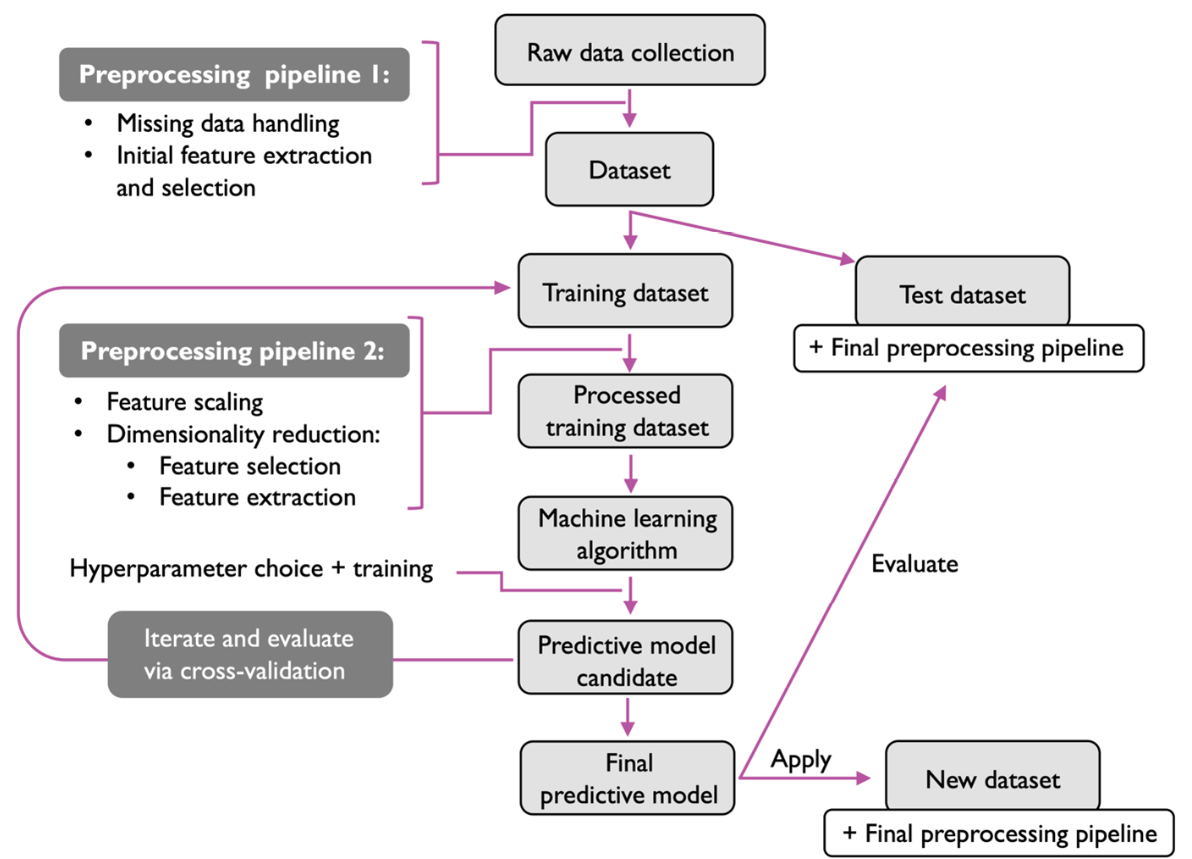
\includegraphics[width=.9 \textwidth]{Figures/ExampleFigure.png}
\caption{Example \label{Fig:Example}}
\end{figure}


\subsection{Stakeholder Characteristics}

Refer to \textit{(Clause 9.6.6, 9.5.4.3, 9.4.5)}

\subsection{Limitations}

Refer to \textit{(Clause 9.6.7)}

\section{Definitions}

You should add acronyms and abbreviations here. Refer to \textit{(Clause 9.6.7)}



For any citation, refer to it as \cite{younis2021hybrid}.
